\chapter{Calibration}
\label{chap:calibrate}
\section{Calibration variables}
The purpose of a hydrodynamic calibration is to ready the model for the domain or application, 
as well as gain insight into its suitability for general modeling purposes.  This insight can then 
be quantified by validating over a longer period in which the model is not adjusted. Calibration 
and validation are always indicated for a new model application; they may also be indicated when 
new physical processes (sediment, biogeochemistry) are added, additional focus
is required of a subarea of the domain or new data becomes available.

This calibration covers hydrodynamic variables (water surface, velocities and cross-sectional flows) as well as salinity.
The calibration does not include temperature, although our collaborators on the SESAME project have done extensive work in the Bay on temperature and we expect to publish results on temperature over the full Delta soon.

Salinity (and conductivity) are among the best monitored constituents in the system. 
Salinity is a conservative tracer, meaning that it is not consumed or created by reactions with other 
constituents, affected by heat flux or interactions with sediment. All conservative tracers 
are transported by the same physical processes, so that in principle a salt calibration should 
apply to other conservative constituents such as bromide or \gls{doc} as well as providing the foundation
for modeling nonconservative constituents such as dissolved oxygen and mercury. Inasmuch as there are
differences between salinity and other constituents this is because of the role of the ocean boundary.
Most salinity in the Delta is carried up the estuary through tidal and estuarine mixing processes such as gravitational circulation. 
With DSM2, the Delta Modeling Section has found it insightful to model \gls{doc} as well, precisely because
is not dominated by ocean sources. This allows a greater focus on other components of transport; it also makes
\gls{doc} more robust to errors in consumptive use estimates.

\section{Calibration parameters}
Although calibration is often liked to turning knobs, the process of calibrating a 3D unstructured 
grid model with ten million or more state variables involves numerous activities that don't amount to parameter adjustment. 
For instance, much of the project development time involves adjusting, refining and balancing the mesh or collecting
and incorporating improved bathymetry. Even when we do adjust the model, selecting or swapping algorithmic options is often more influential than, say, adjusting friction. 

Although we did some experiments with other parameters, the main items that we manipulated in the calibration were these:
\begin{itemize}
	\item horizontal mesh configuration and density
	\item vertical mesh selection, configuration and density
	\item roughness coefficients
	\item the selection of turbulence closure
	\item the choice between higher order and linear ELM
\end{itemize}

We experimented with several relationships between roughness or drag and depth, but we applied the same formulas
over the entire domain -- we did not consider spatially varying friction formulas. 
Using different roughness or even different turbulence closure might be appropriate for based
on the presence of bedforms or vegetation, but these distinctions would involve additional data collection and 
introduce seasonality. We may visit these ideas in the future for detailed study regions where more complete observations are available concerning horizontal and vertical velocity structure and lateral distribution of tidal phase.


\section{Calibration period and time step}
The period of the the calibration period covered in this document is March 12, 2009 to ****, 2010. The year 2009 is categorized as Dry and 2010 is categorized as Below Normal. We used the period March 12, 2009 as the start date because of the availabilty of USGS cruise data for salinity initial conditions.
The period through Fall 2009 was used as the basis of adjusting parameters. The bulk of 2010 was used for validation.

The hydrodynamics time step is 120 seconds for all the simulations. This time was decided early in the project on the basis of sensitivity runs on the Bay-only variant of the mesh and is in keeping with the 
\gls{cfl} minimum time step to avoid numerical diffusion in the the Eulerian-Lagrangian 
component of the algorithm (see section ***). The scalar transport 
part of the code is based on a different CFL time step restriction, this one a maximum rather than a minimum, 
and as a result the transport regularly subcycles the main hydrodynamic time step using steps between 3 and 20 seconds.

\section{Skill metrics for scalar station data}
For station observations of scalar quantities such as stage and flow, 
we evaluated model performance based on both visual assessments of time series plots and 
quantitative fitness scores. 

Each station analysis includes 14-day dynamic plots revealing tidal characteristics 
at the site over spring and neap conditions, as well as longer plots of tidally filtered results showing the
system response to longer period fluctuations such as barometric events and seasonal
inflow changes. For the tidally filtered plots, infrequent small gaps 
in the observed records were filled using interpolation in order to avoid the widening 
of the gaps to days that occurs when missing data are filtered. 

Below the time series plots are scatter plots of the phase-adjusted model results 
and observed data fitted with a regression line. The slope of the regression line has been
described by \cite{MacWilliams08} as a measure of signal amplitude amplification for tidal oscillations
and by \cite{Murphy88} as a measure of conditional bias (e.g., flow bias that grows or shrinks with flow).  
We also record the correlation coefficient (the square root of ${R^2}$) for consistency with other models
that also record this statistic. We do this with some hesitation given the shortcomings of the statistic in the current context
-- for serially correlated data this statistic occupies a narrow scale \cite{Ralston2006}, neglects important aspects of fit
\citep{Murphy88}. It also may give false positives or medium-high scores for nearly random predictions \citep{Ralston2006}
and does not appear to be informative in the presence of patterned errors such as would occur in a tidal environment. 

The scale of the scatter plots gives a good indicator of the total variability in the data 
including both tidal and non-tidal components. It can be contrasted with the scale of the 
tidally-filtered time series plots, whose y-axis is a good indicator of the variability of
the subtidal part of the signal. The scale of the dynamic plots was a compromise -- we used the 
natural range of the dynamic period data but constrained the range to be at least as large 
as that of the filtered data. 

We also evaluated fitness scores for important aspects (bias, fit, skill, phase) of 
model performance. The following statistics are reported where
appropriate:

\begin{description}
  \item{{\textbf{RMSE}}} Root mean square error. Note that unlike the other statistics 
	below marked with a $\phi$ subscript (and published calibrations from other models), 
	the data are not phase-corrected for this statistic.
  \item{{\textbf{Lag}}} An estimation of lag based on cross-correlation analysis, 
	similar to that described in RMA (2005) \cite{RMA05}. The idea of this analysis is to shift
	the model results forward and backward in time until the maximum cross-correlation 
	between the two series is obtained. A positive lag indicates that the model trails the
	field observations in the timing of tidal signals. The effectiveness
	of this statistic depends on the strength of the tidal signal compared to noise and longer term trends with vague     
	periodicity. The analysis was not performed for Delta salinity stations.
	\item{\textbf{Bias}\subphi} The median bias  of phase corrected error (modeled - observed)
	\item{\textbf{NSE}\subphi} The Nash-Sutcliffe efficiency for the phase-corrected error:
	\begin{gather}
	NSE\subphi(f,r,x) = 1 - (MSE(f,x)/MSE(r,x)) \\
	\text{where} ~ MSE(f,x) = \frac{1}{n} \sum\limits_{i=1}^{n}(f_i - x_i)^2 \\
	\end{gather} is the mean squared error between a forecast ($f$), an observation ($x$) 
	and a {\em reference forecast}. The choice of 
	reference forecast can several possible skill scores -- 
	the Nash-Sutcliffe is the simplest with $r$ representing the station time-average.
	\item{\textbf{r}\subphi} The correlation coefficient (the $r$ in $R^2$ for the fit 
	of the observations on the phase-corrected model values.
\end{description}


In addition to covering the major facets of accuracy in a tidal
system, the main criteria for these metrics were robustness and consistency with
other Bay-Delta model calibrations. The variety of published skill metrics for hydraulic and hydrologic models is extensive 
(some examples are \citet{Willmott82,Willmott85,Willmott12}, \cite{Stow09}, \cite{Murphy88}, \cite{Ralston2006}). 
No standard has emerged \citep{Stow09}, and there seems to be some schism between practitioners who work with 
measures of accuracy (e.g. RMSE) and those who work with skill. 

For systems with periodic forcing such as an estuary, many of the above statistics are sensitive to the phase 
(time shift) of the model relative to the observations. If this error is not controlled, 
it reduces the diagnostic value of the suite because the statistics would not differentiate an excellent
tidal signal with a modest shift from a shabby tidal signal. 
Following  RMA (2005) \cite{RMA05}, we first estimate phase error and then correct for phase (by shifting the model output in time) 
when generating the remaining statistics except for RMSE which is left as a composite indicator of overall error.

The metrics are not decomposed into tidal and subtidal time scales. This means that the diagnostic 
that the underlying physics and time series plots do. Subtidal and tidal information can therefore
obscure one another. In particular, tidal signals are generally much larger than the variation
of longer period fluctuations. When the two are mi

\section{Station inventory and descriptions}
The locations of stage, flow and salinity stations is shown in Figures ***. 
We relied on data from the following agencies and programs (method of retrieval is shown in parentheses):

\begin{itemize}
  \itemsep1pt \parskip0pt \parsep0pt
	\item NOAA (automated retrieval)
	    \subitem Verified Water Levels from ***
			\subitem Conductivity at *** stations in the Bay.
	\item USGS (request)
	    \subitem Conductivity from the Water Quality and Sediment *** Group
			\subitem Flow, stage and (post-2010) water quality from the Delta Hydrodynamics Group in West Sacramento
			\subitem CTD (conductivity-temperature-depth) cast data from cruises conducted by ***
  \item CenCOOS surface HF Radar
	\item DWR North Central Regional Office or NCRO (Water Data Library) 
	    \subitem Flow
			\subitem Surface Water Monitoring Program
			\subitem Water Quality Monitoring Program
	\item DWR Compliance* and IEP (request) for conductivity monitoring at **** sites
	\item DWR O\&M (CDEC) for operational data and pumping rates
	\item USBR (CDEC) conductivity and temperature stations in the Delta
\end{itemize}

In each case we report the station name, agency identification and CDEC identification for familiarity. 
\vfill
\section{Stage Results}
	   
  \subsection{Monitoring stations}
  \subsection{Tidal phase and amplitude}
	  Figures \ref{fig:m2_amp} - \ref{fig:k1_phase} map the evolution of the two 
		largest tidal constituents, M2 and K1, through the Bay-Delta 
		system for both model and observations during the month of ***. The amplitudes are labeled in meters, 
		phase is in terms of minutes difference from the timing at the Golden Gate. 
		
		The development of the tide through the Bay is generally accurate for M2; 
		there is an 11 minute delay in K1 at the San Francisco 
		station ***** but accuracy is good at most stations.
		
		Upstream in the Delta, there is a tendency for the tide to be underdamped -- the model overestimates 
		tidal amplitude and is early for phase at most stations. The error is regionally consistent, 
		meaning that stations nearby one another in the Sacramento, San Joaquin, 
		and Old and Middle River regions have similar characteristics. 
		Dampening can be increased roughness or by use of linear interpolation at the feet of characteristics
		in ELM, which is diffusive, but either measure entails reduction in the tidal range of flow. 
				

\begin{figure}
	\centering
		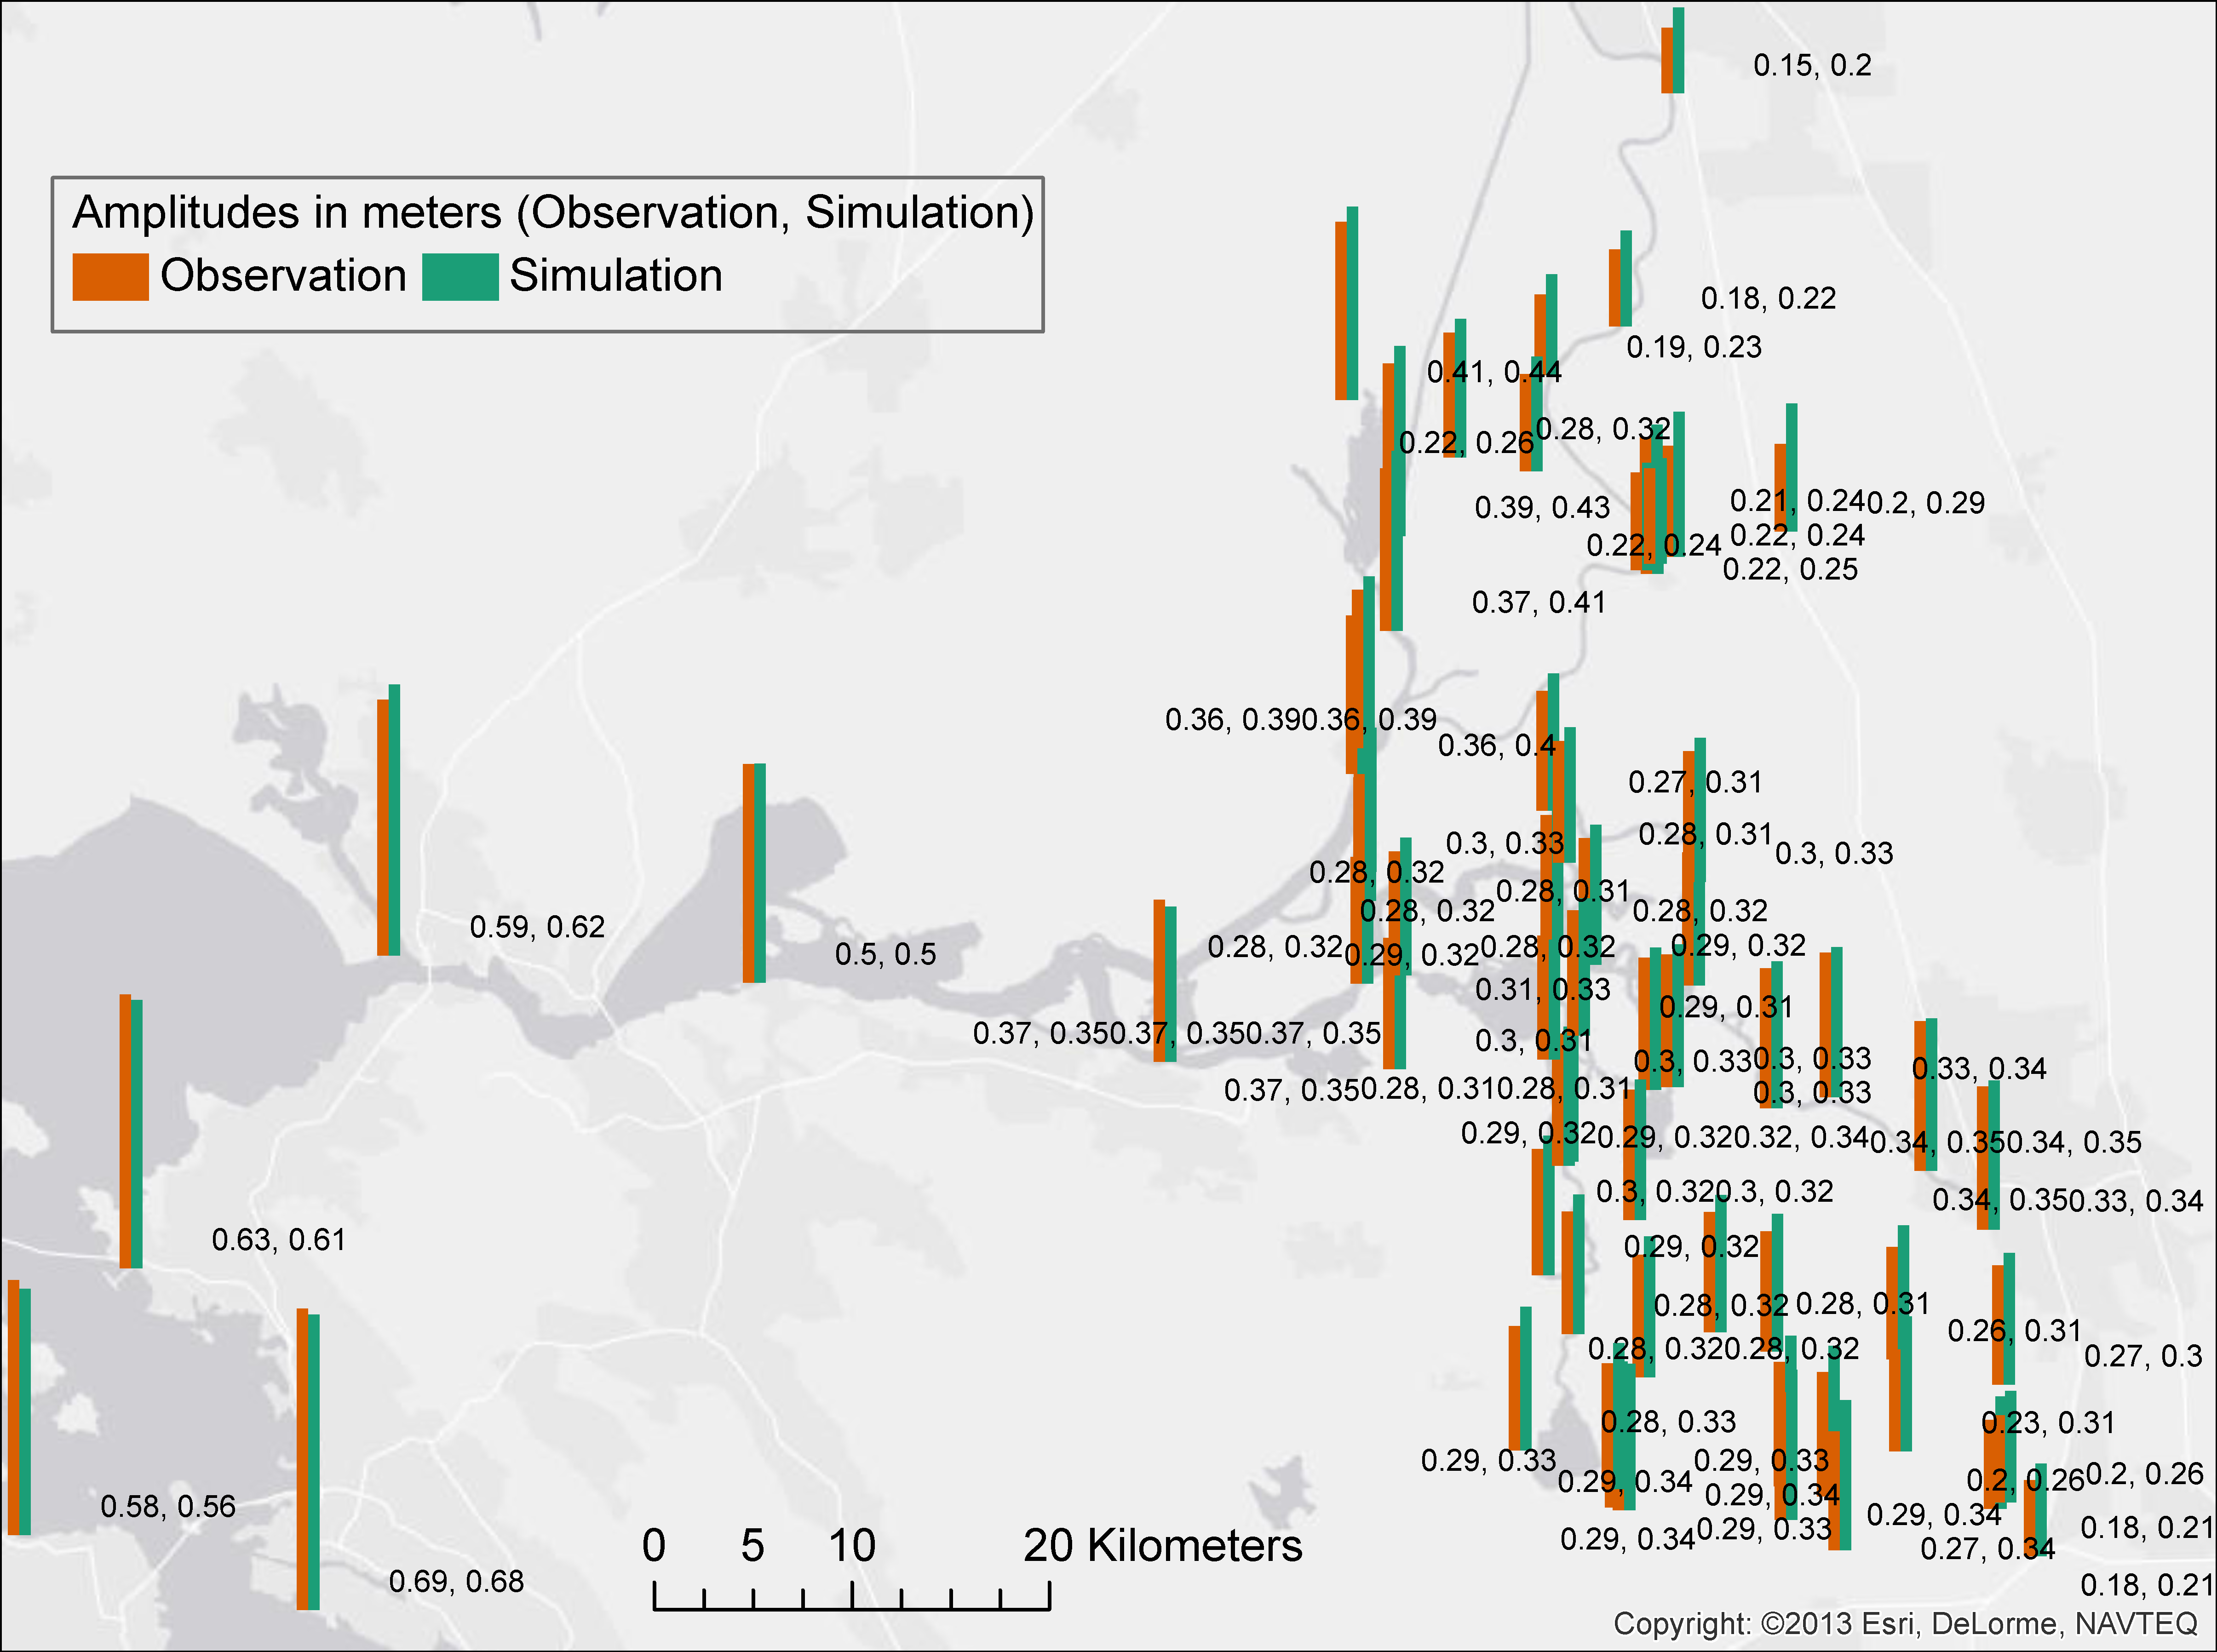
\includegraphics[width=\textwidth]{image/M2_amp_spatial}
	\caption{Map of M2 amplitude at Bay-Delta stations.}
	\label{fig:m2_amp}
\end{figure}
\begin{figure}
	\centering
		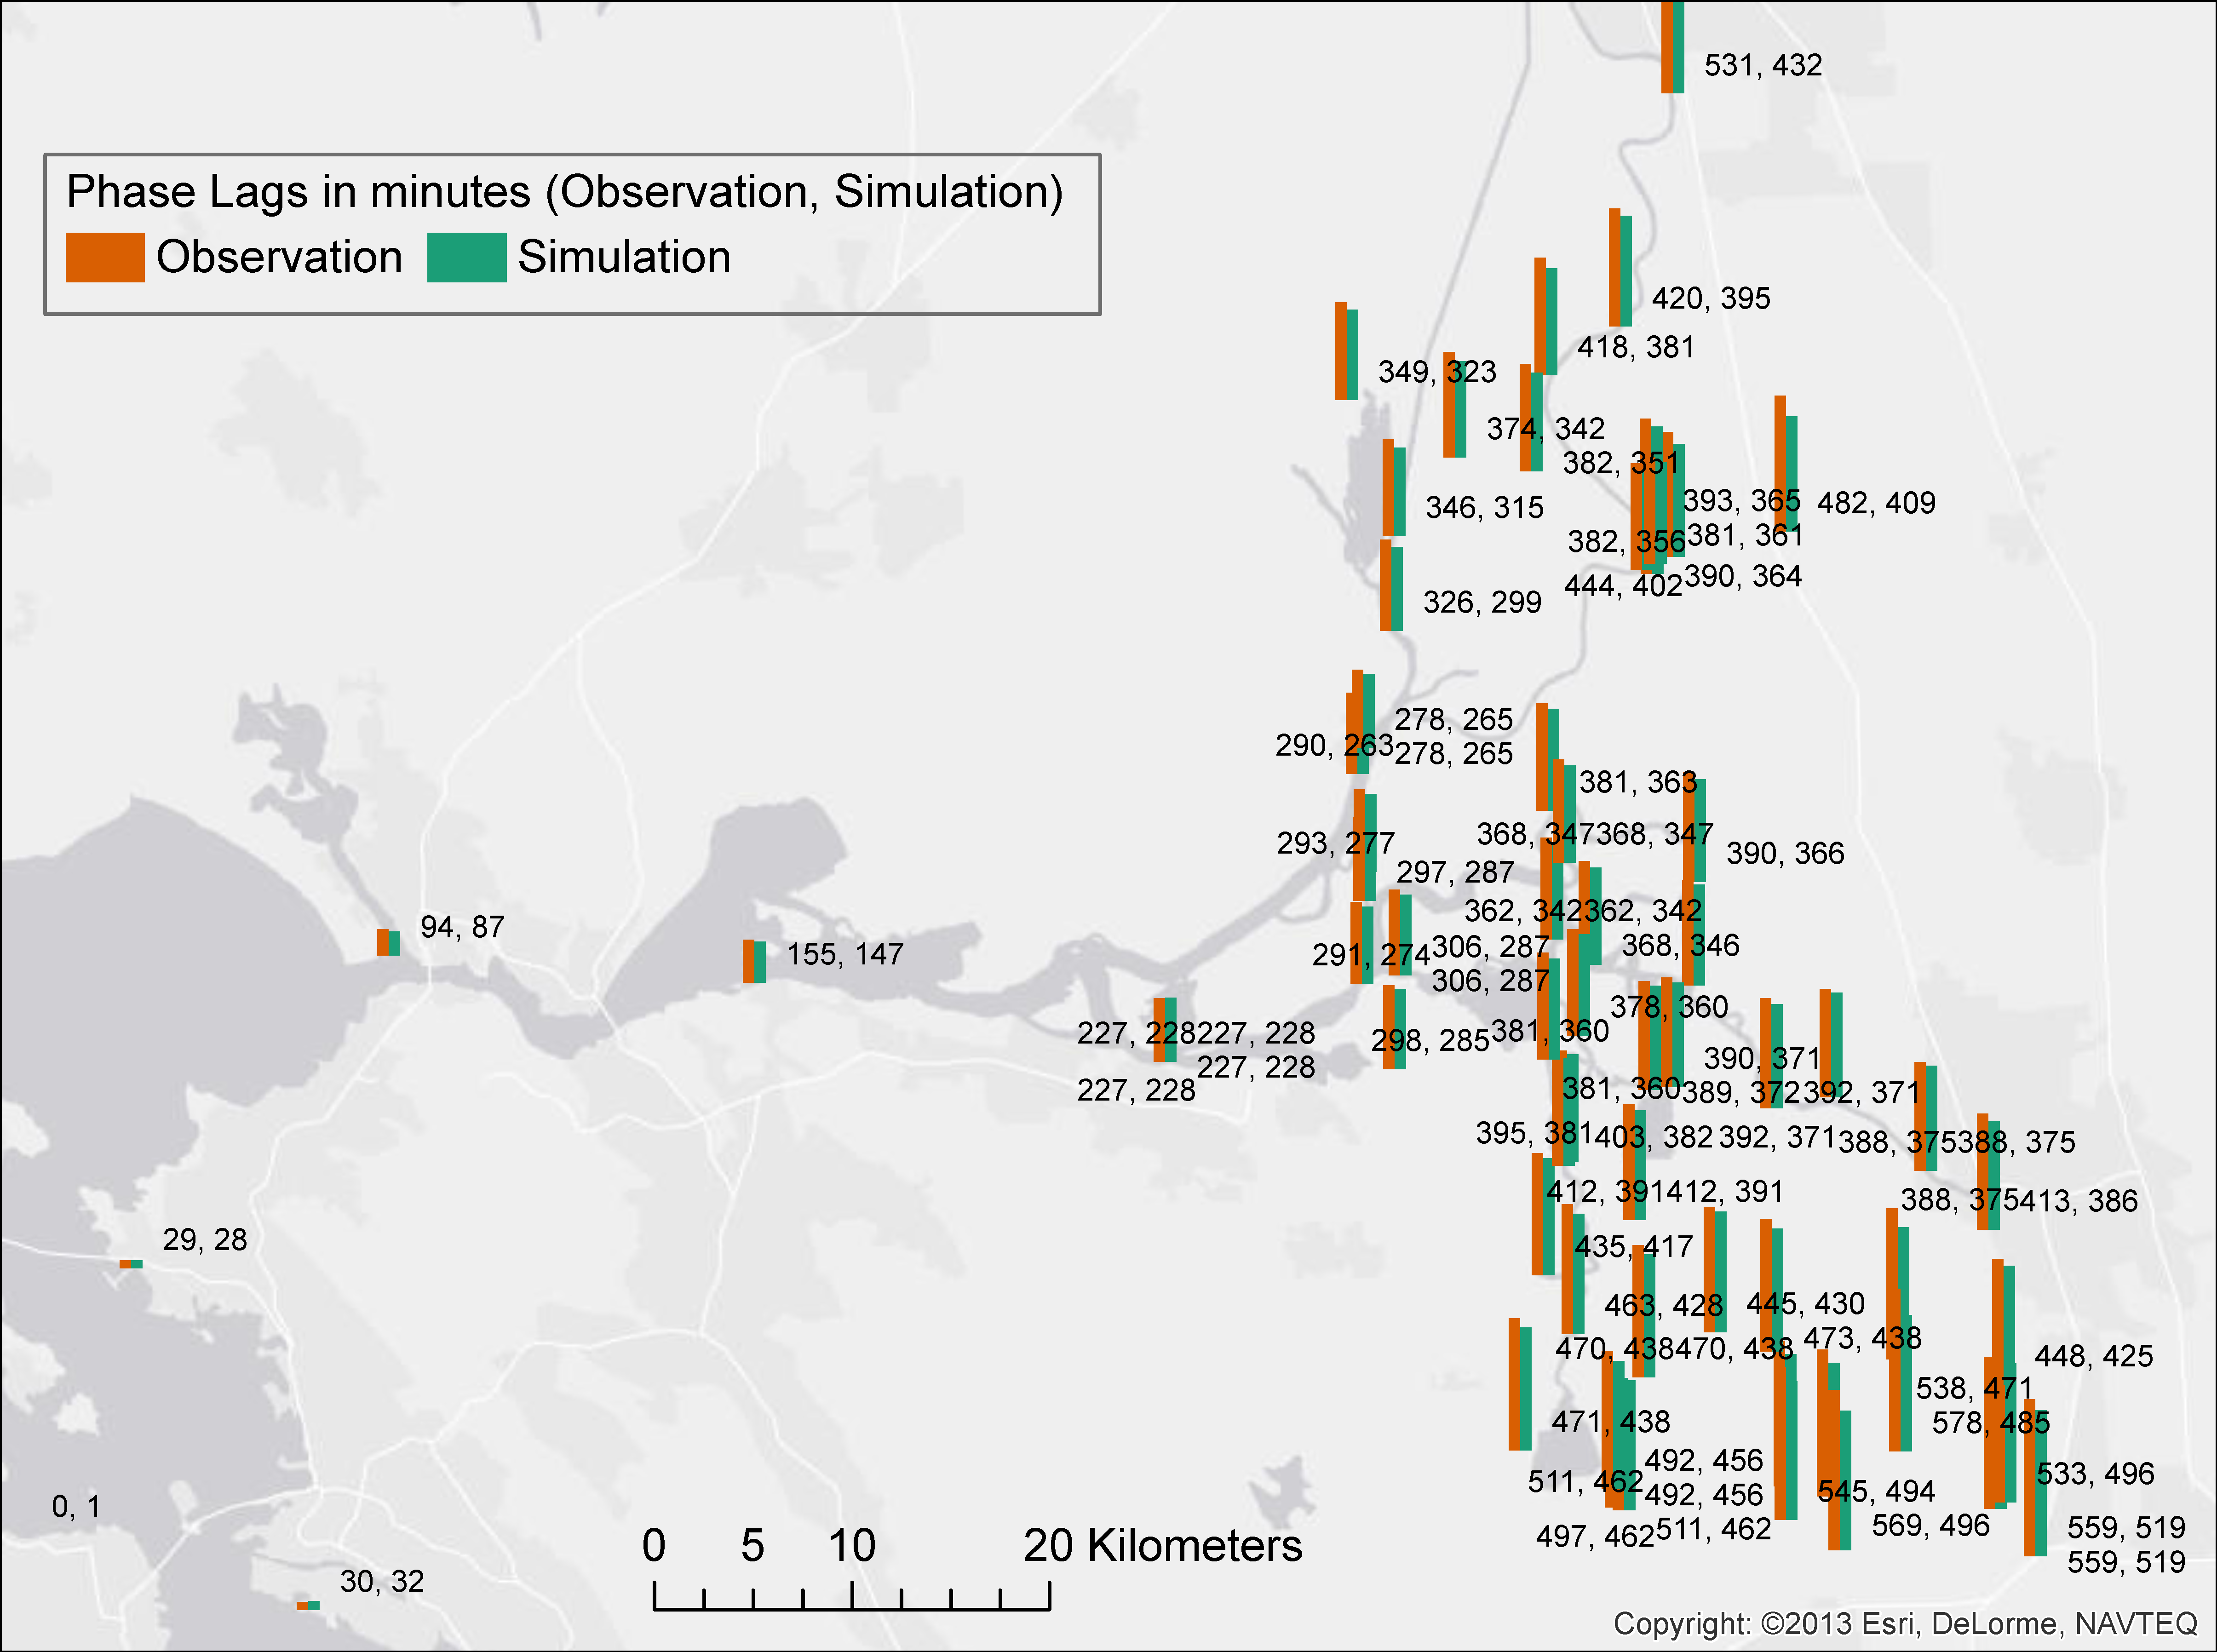
\includegraphics[width=\textwidth]{image/M2_phase_min_spatial}
	\caption{Map of M2 phase at Bay-Delta stations.}
	\label{fig:m2_phase}
\end{figure}
\begin{figure}
	\centering
		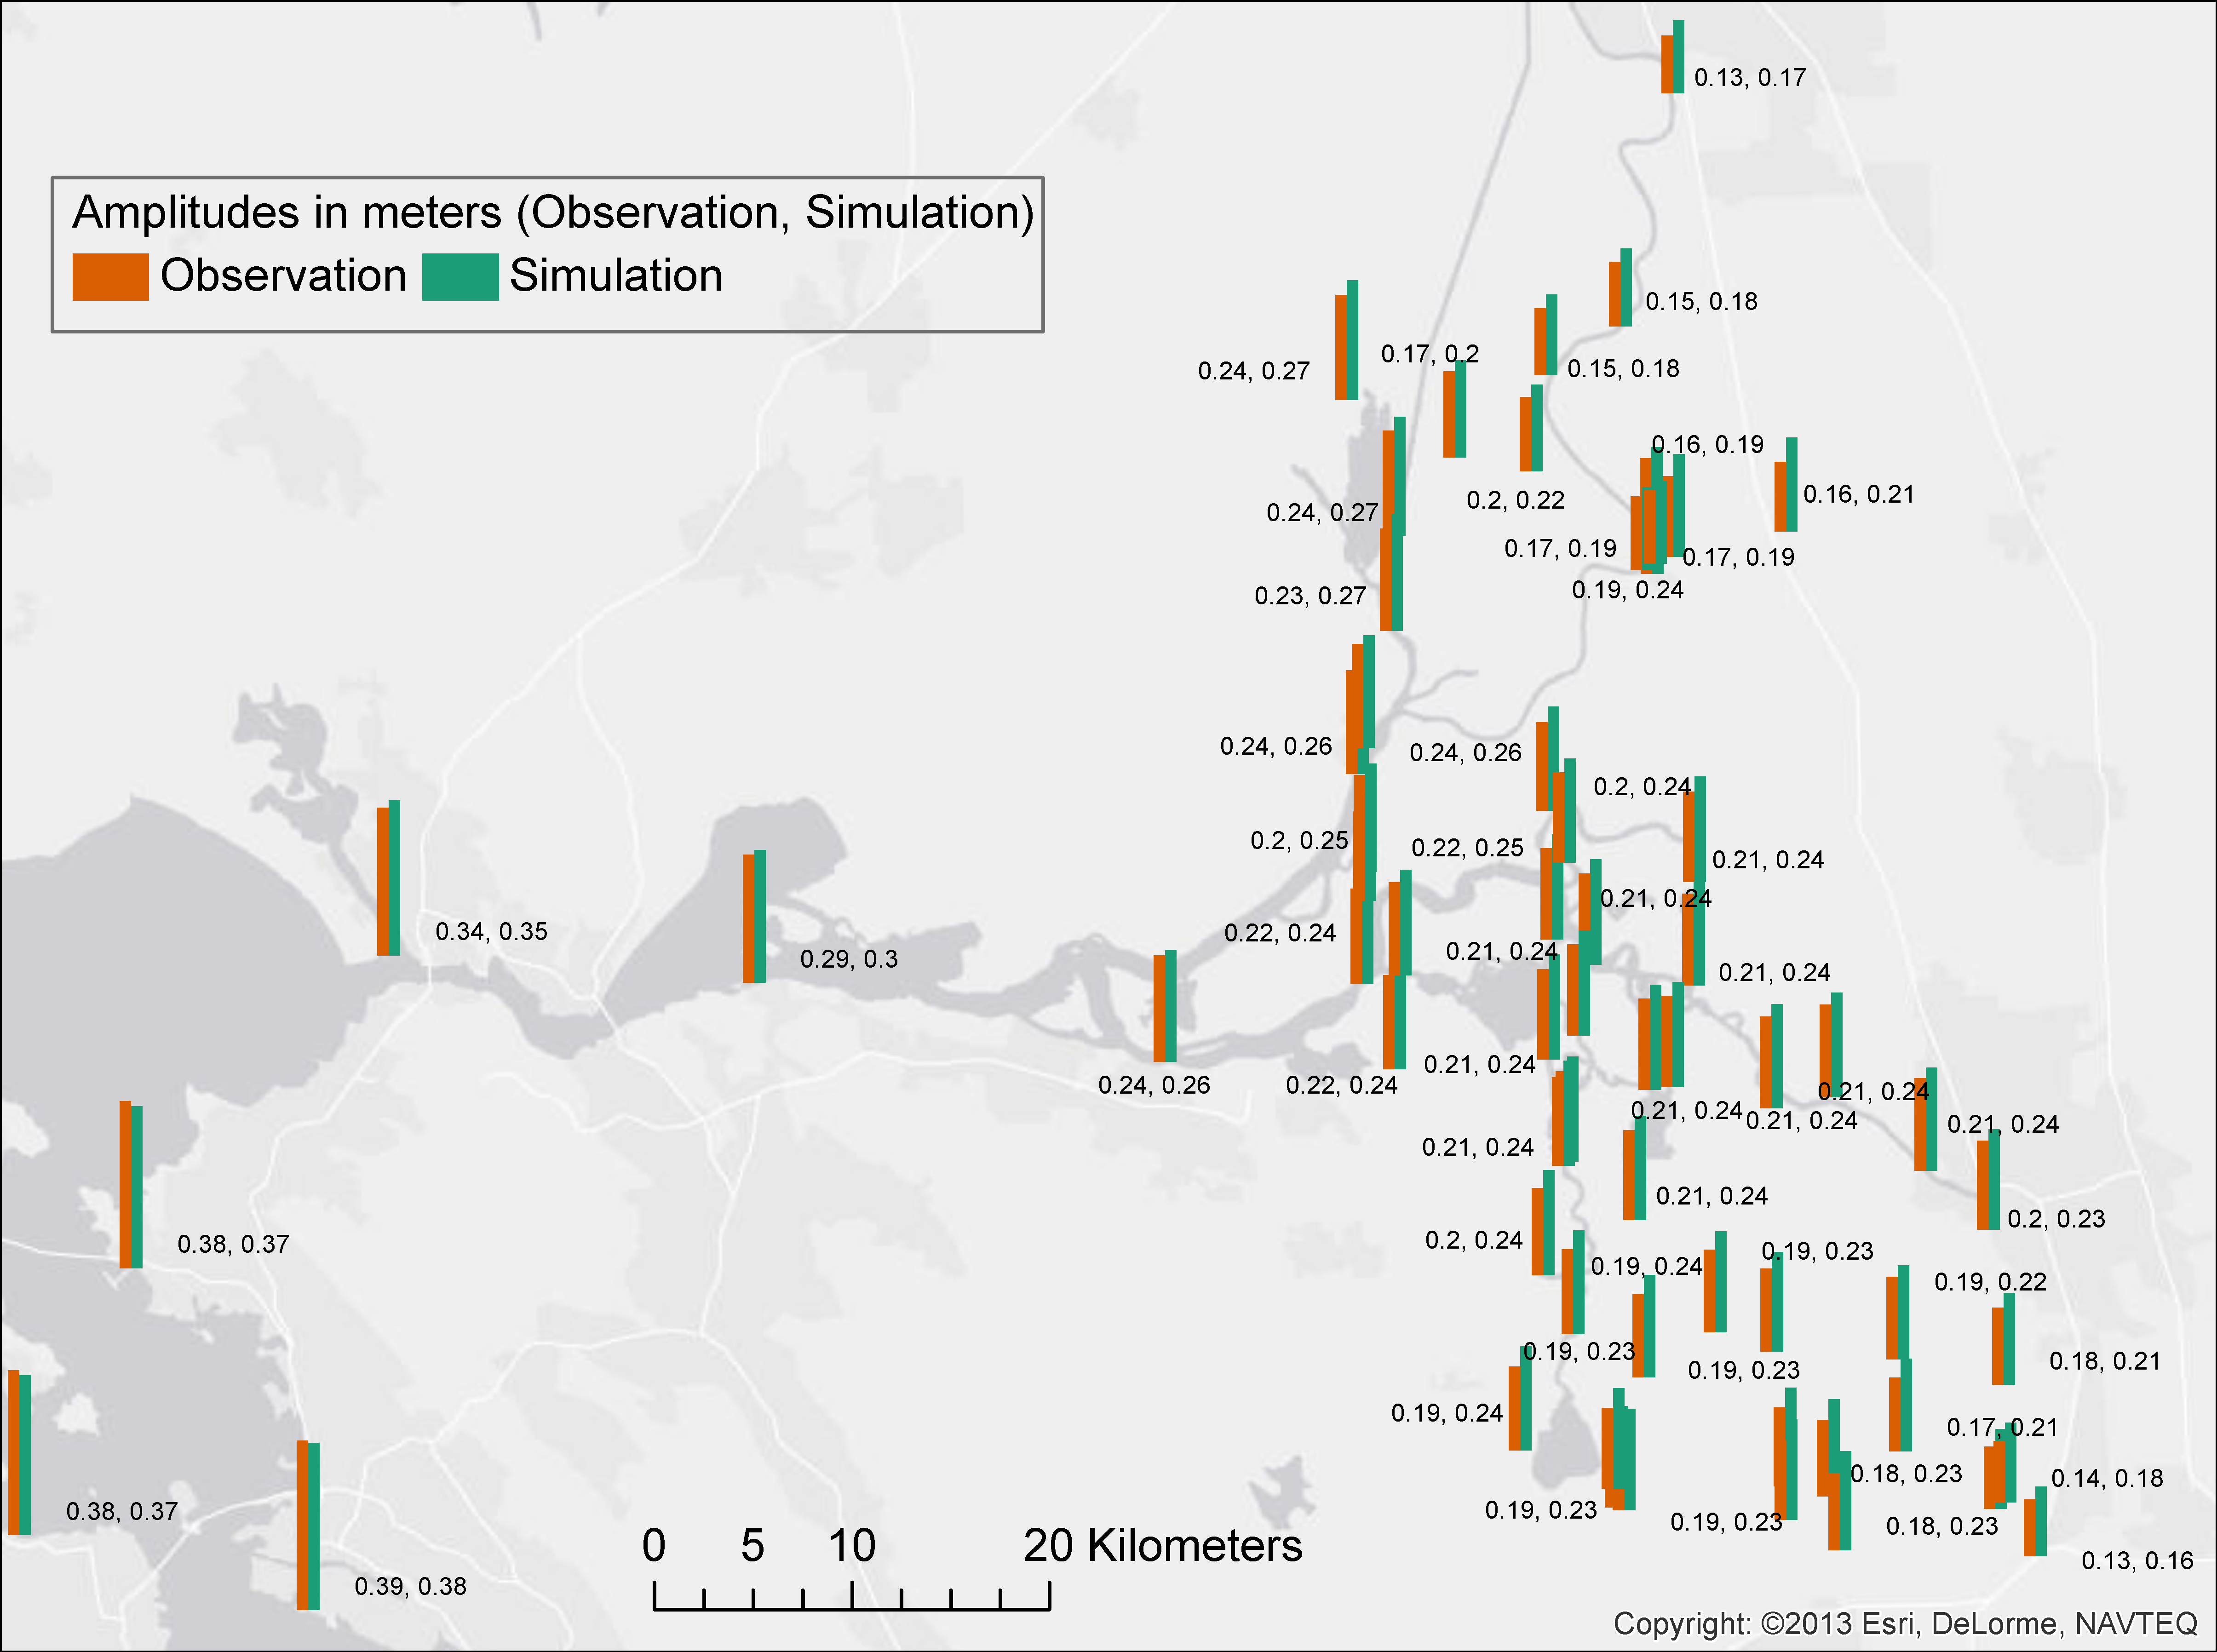
\includegraphics[width=\textwidth]{image/K1_amp_spatial}
	\caption{Map of K1 amplitude at Bay-Delta stations.}
	\label{fig:k1_amp}
\end{figure}
\begin{figure}
	\centering
		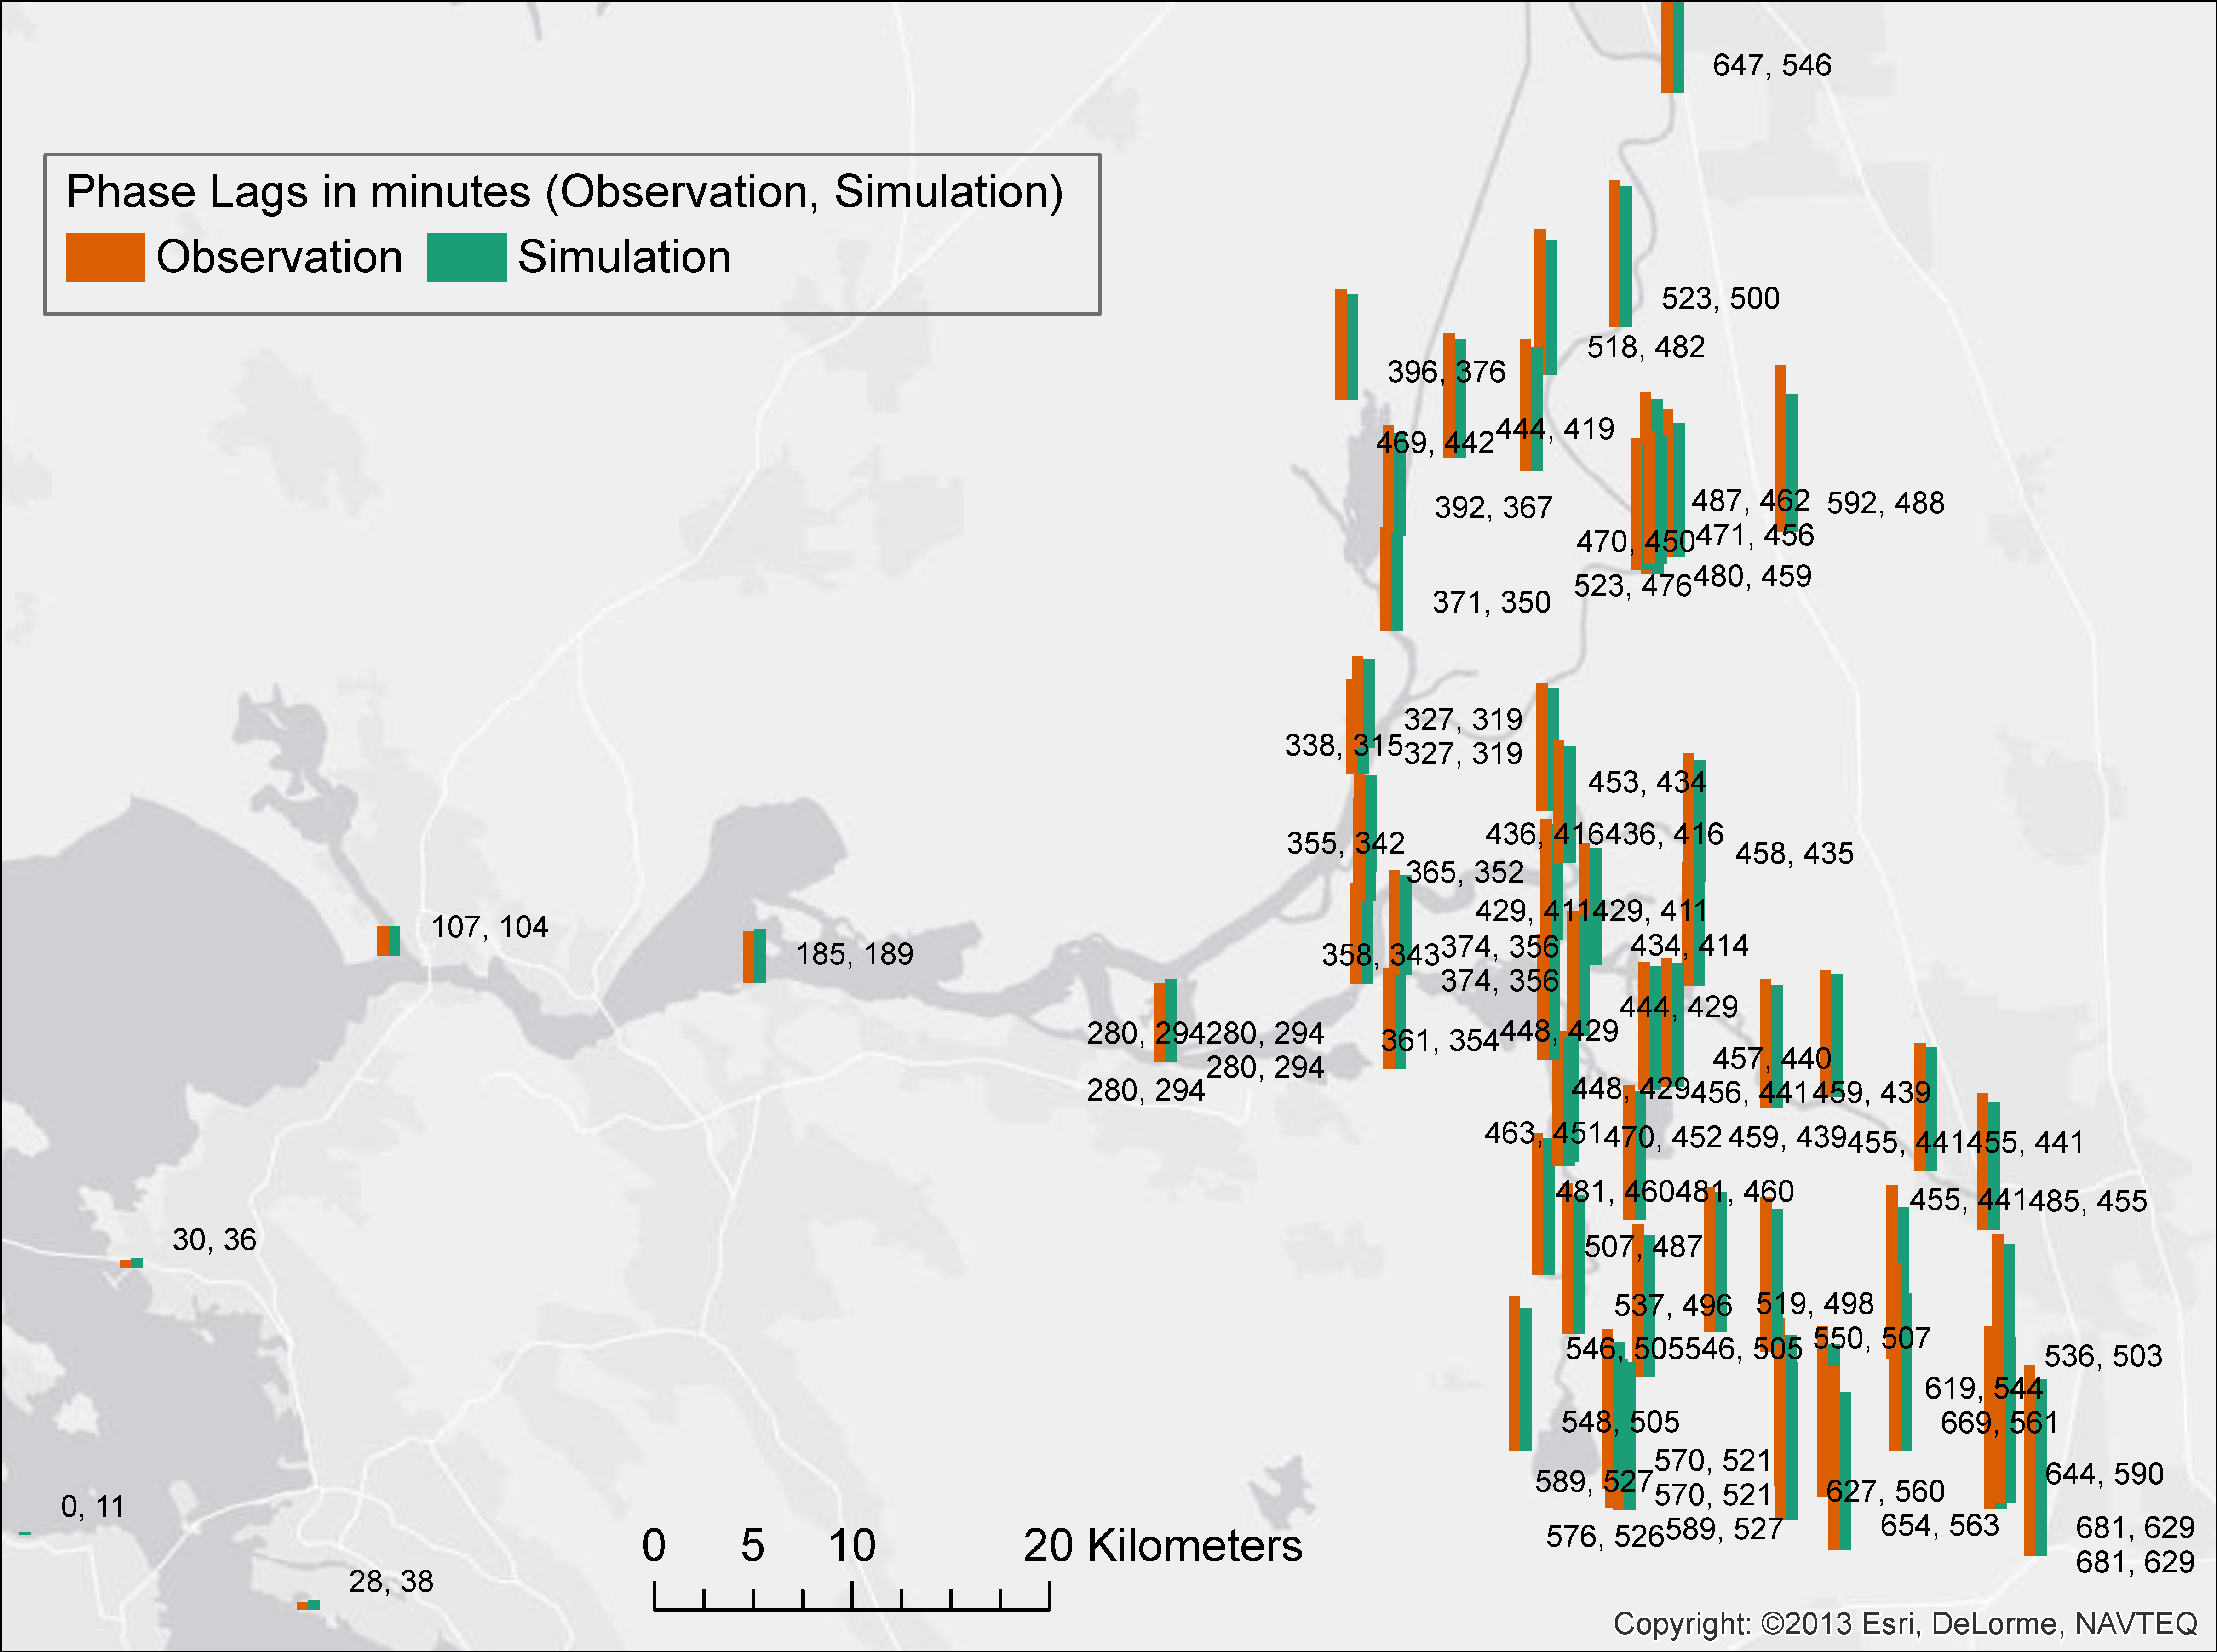
\includegraphics[width=\textwidth]{image/K1_phase_min_spatial}
	\caption{Map of K1 phase at Bay-Delta stations.}
	\label{fig:k1_phase}
\end{figure}

		
		
\section{Flow Results}
  \subsection{Monitoring stations}
	\subsection{Net flow maps} Net flow maps help give a synoptic view of circulation in the Delta. 
	{\em Net flow} here refers to residual flows after filtering to eliminate tidal frequencies 
	or spring-neap variation. Residual flow is of some direct interest because it can contribute 
	to transport and residence time in the Delta -- though this contribution can . 
	Residual flow is also a diagnostic of how well we can model the details of tidal processes,
	since residual flow often manifests as small systematic asymmetries over a (much larger) tidal pattern. 
	
Figures \ref{fig:resid_north_may}-\ref{fig:resid_south_may} compare model and observed mean flow in the North, Central and South Delta for the month of May, 2009. The averages are taken over one month in order to span a spring neap cycle. Barriers have not been installed at this time in the South Delta.

  The general agreement of model with observations is good, although there are some discrepancies
	in the Franks Tract region. Much of the disagreement has to do
	with the routing of residual flow through Dutch Slough versus Jersey Point. The Dutch Slough
	station AFFRA flow meter in place between May and November 2009 was problematic and was replaced 
	after only six months of deployment.
	
	Many of these issues affect observed data as well. In their calibration document, \cite{RMA05} 
	note that mass balance checks around Franks Tract often have discrepancies of 25 cms (roughly 1000 cfs).
	There is nothing about the DWR or USGS data collection processes that considers mass balance, and the 
	net flow is often a somewhat 
	
	
	since 
	and our
	own flow balances calculations agree with the remarks of \cite{RMA05} that observed 
	
	
\begin{figure}
	\centering
		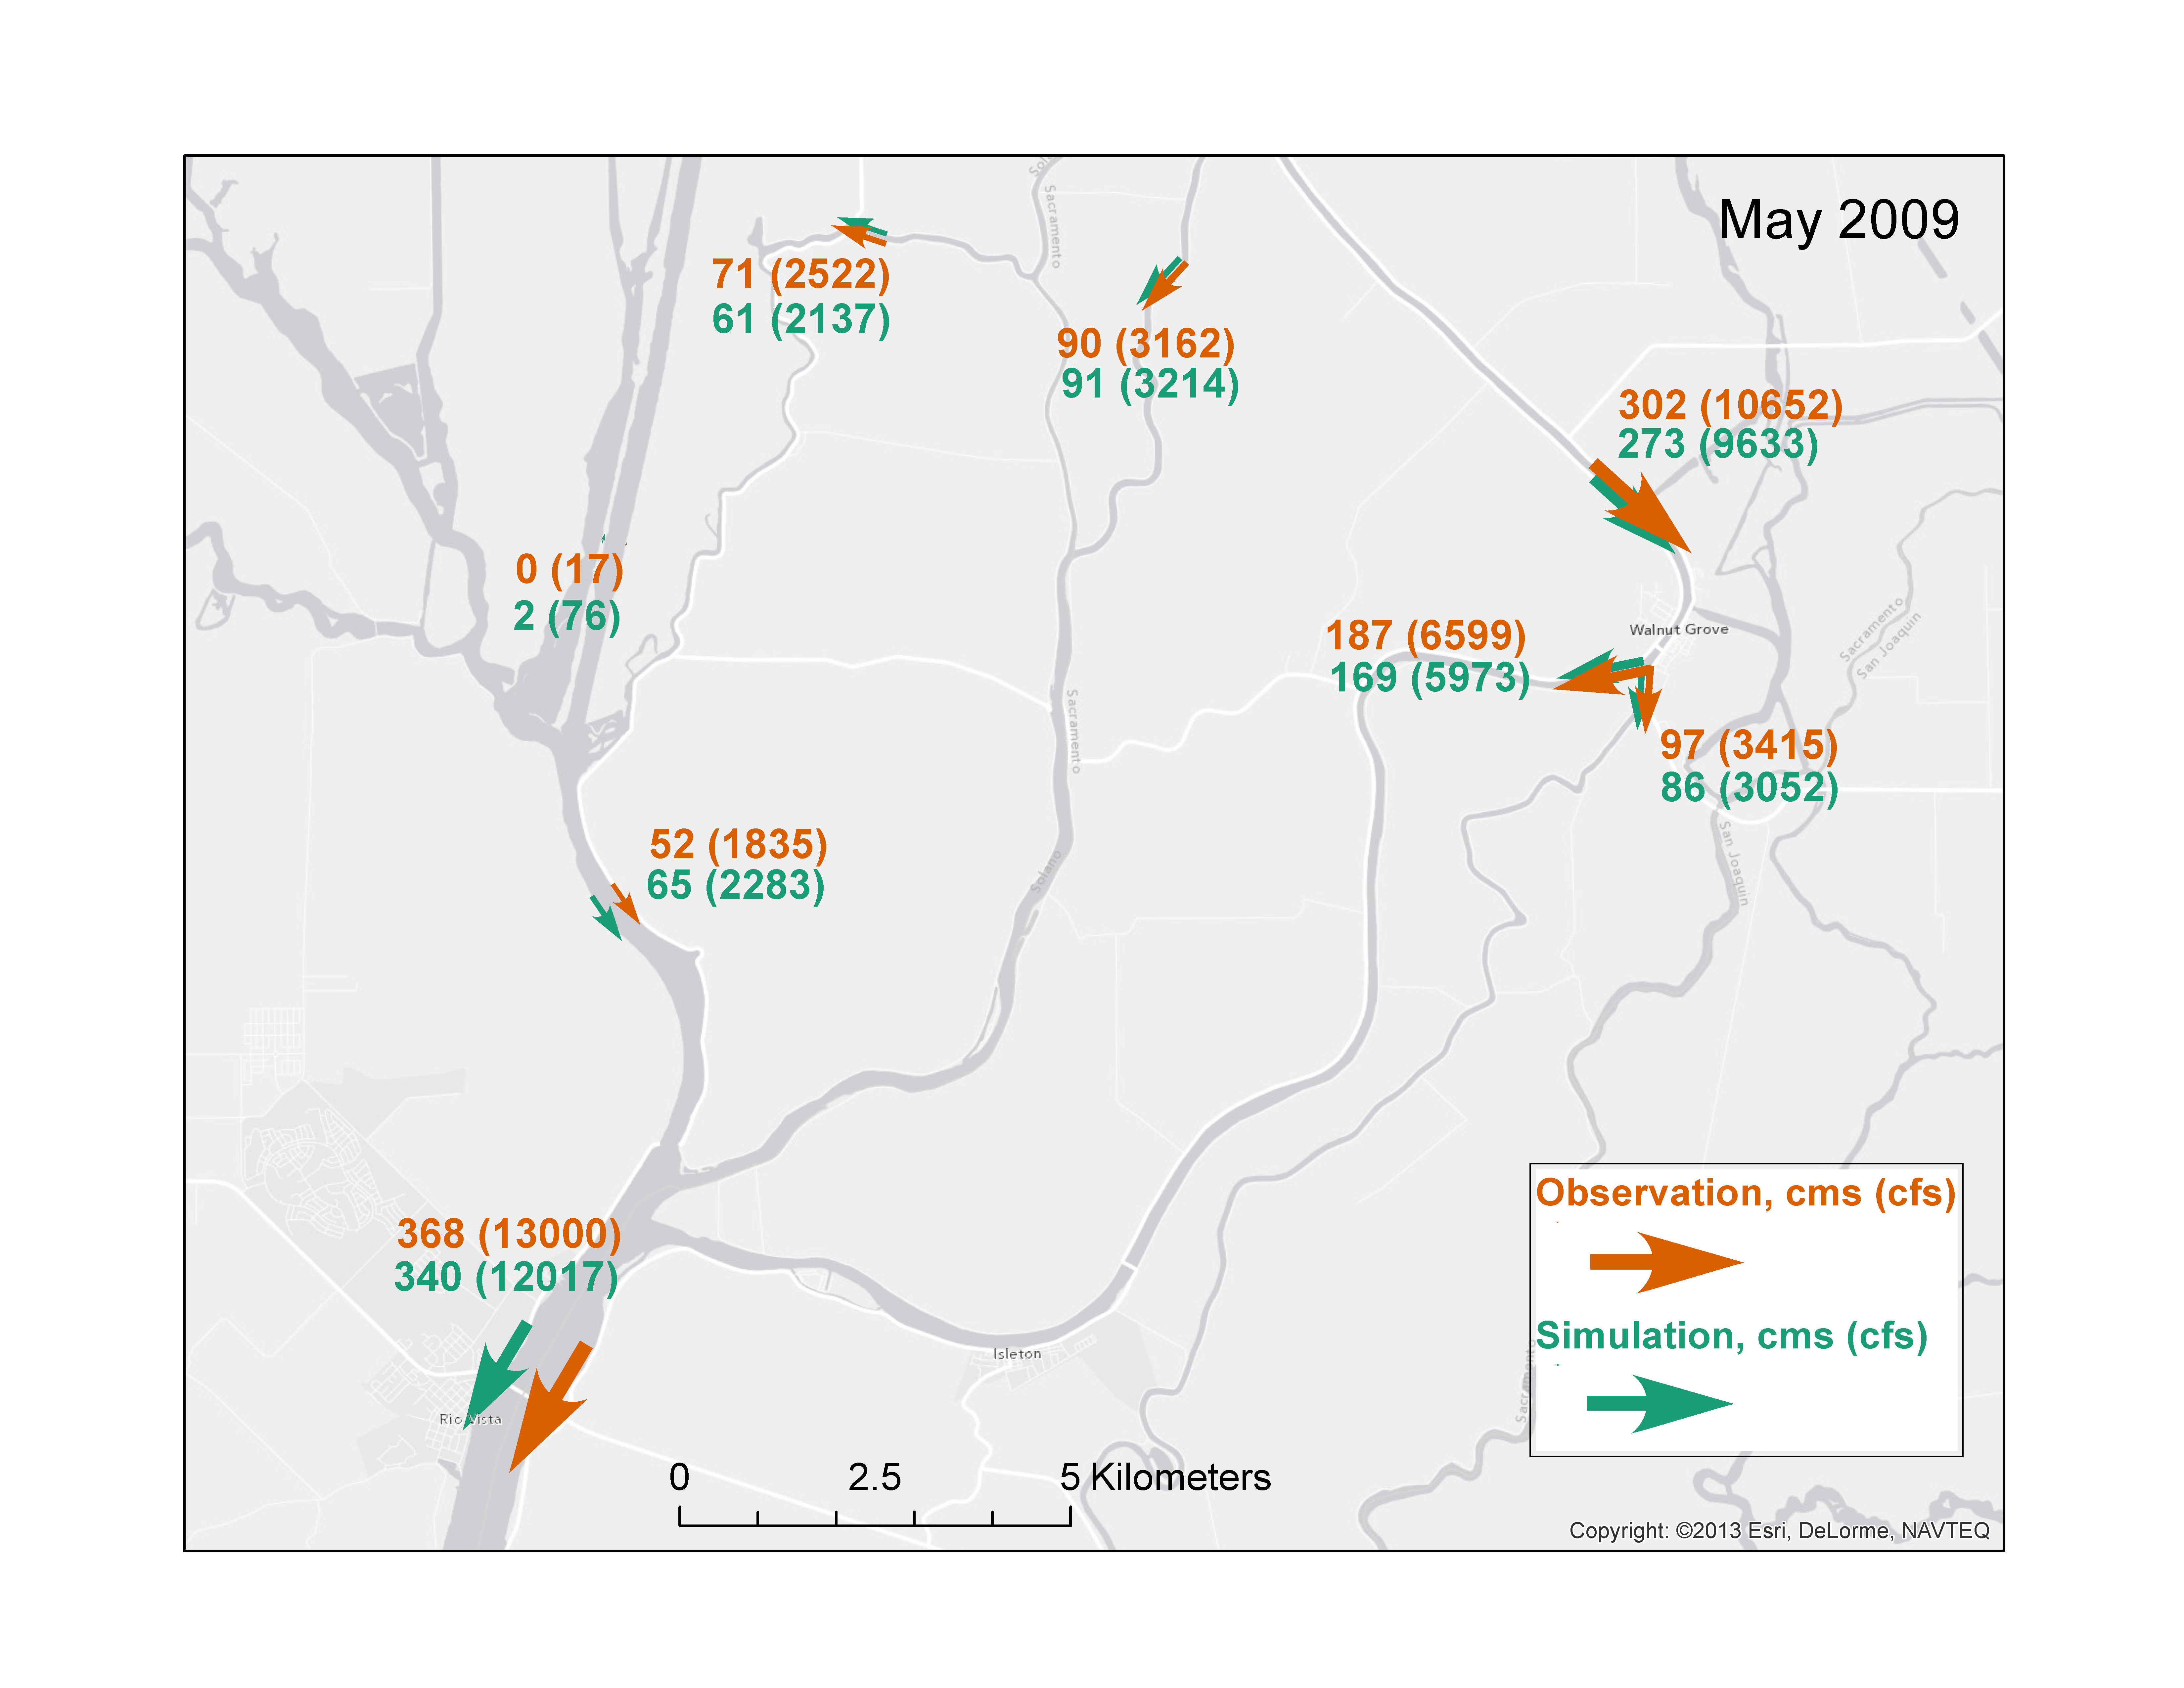
\includegraphics[width=\textwidth]{image/residual_flow_north_delta_64a_may}
	\caption{North Delta monthly residual flow, May 2009. Units are cms (cfs in parentheses).}
	\label{fig:resid_north_may}
\end{figure}

	
\begin{figure}
	\centering
		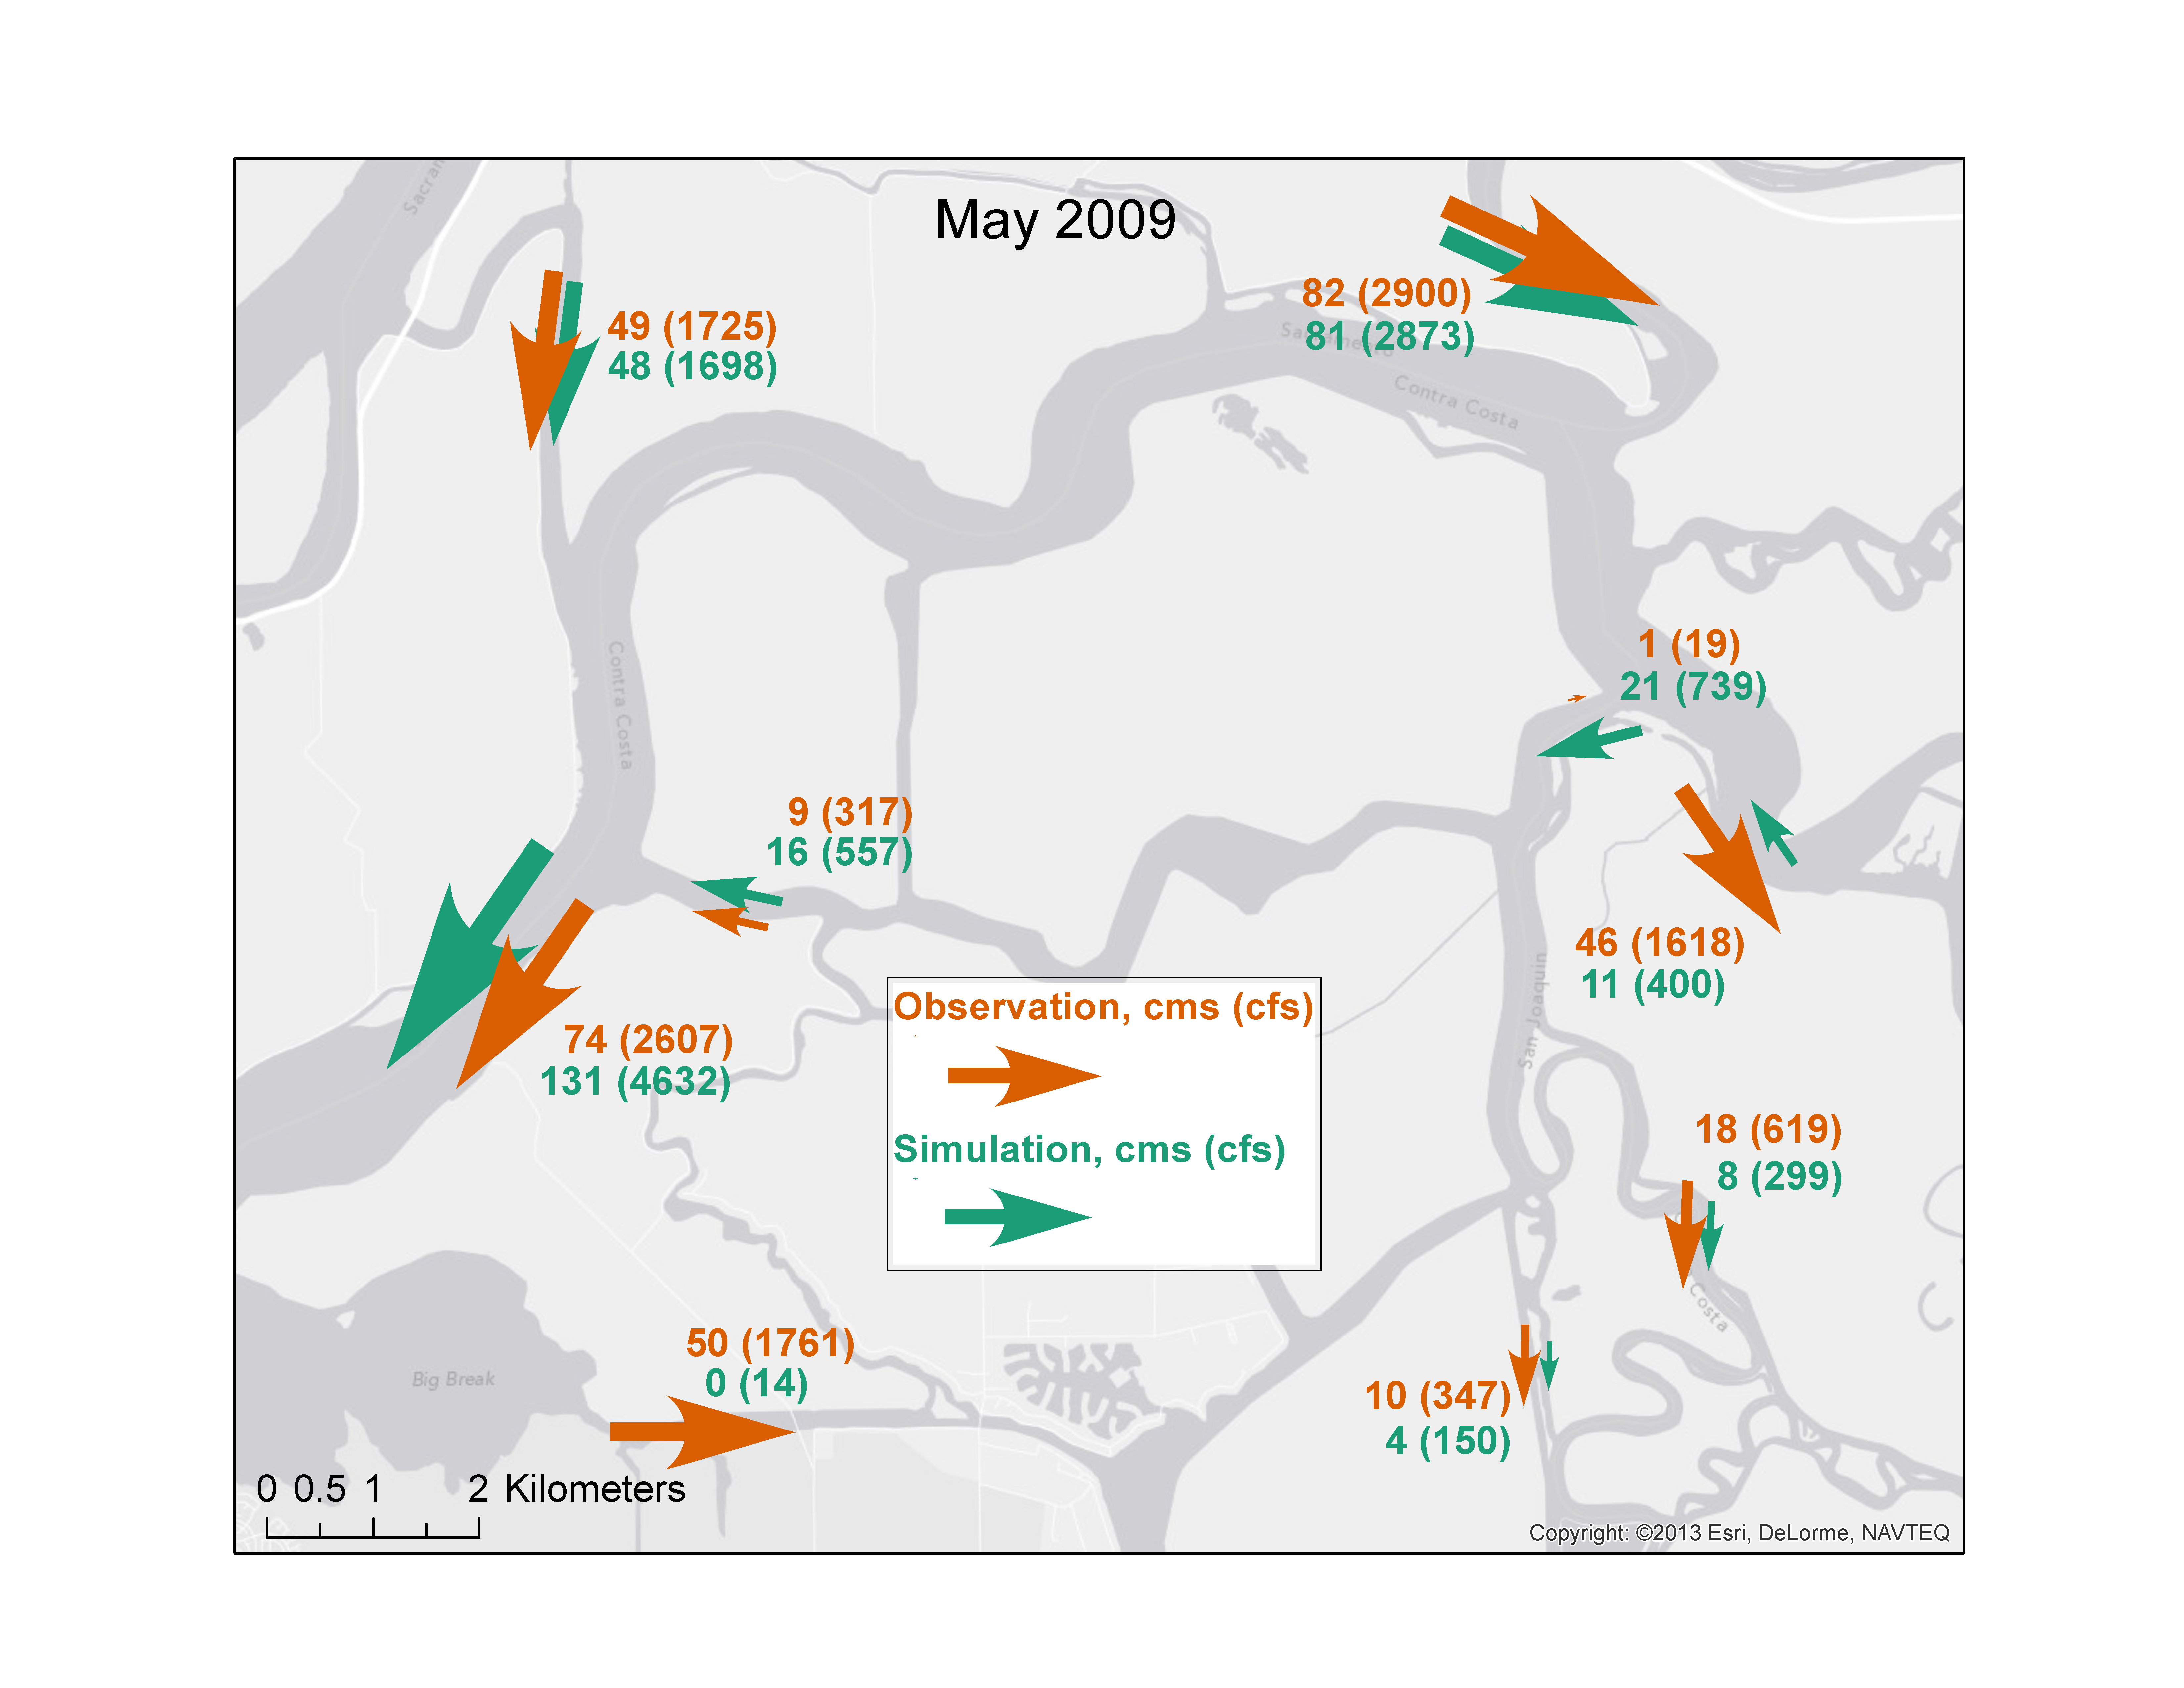
\includegraphics[width=\textwidth]{image/residual_flow_central_delta_64a_may}
	\caption{Central Delta monthly residual flow, May 2009. Units are cms (cfs in parentheses).}
	\label{fig:resid_central_may}
\end{figure}

\begin{figure}
	\centering
		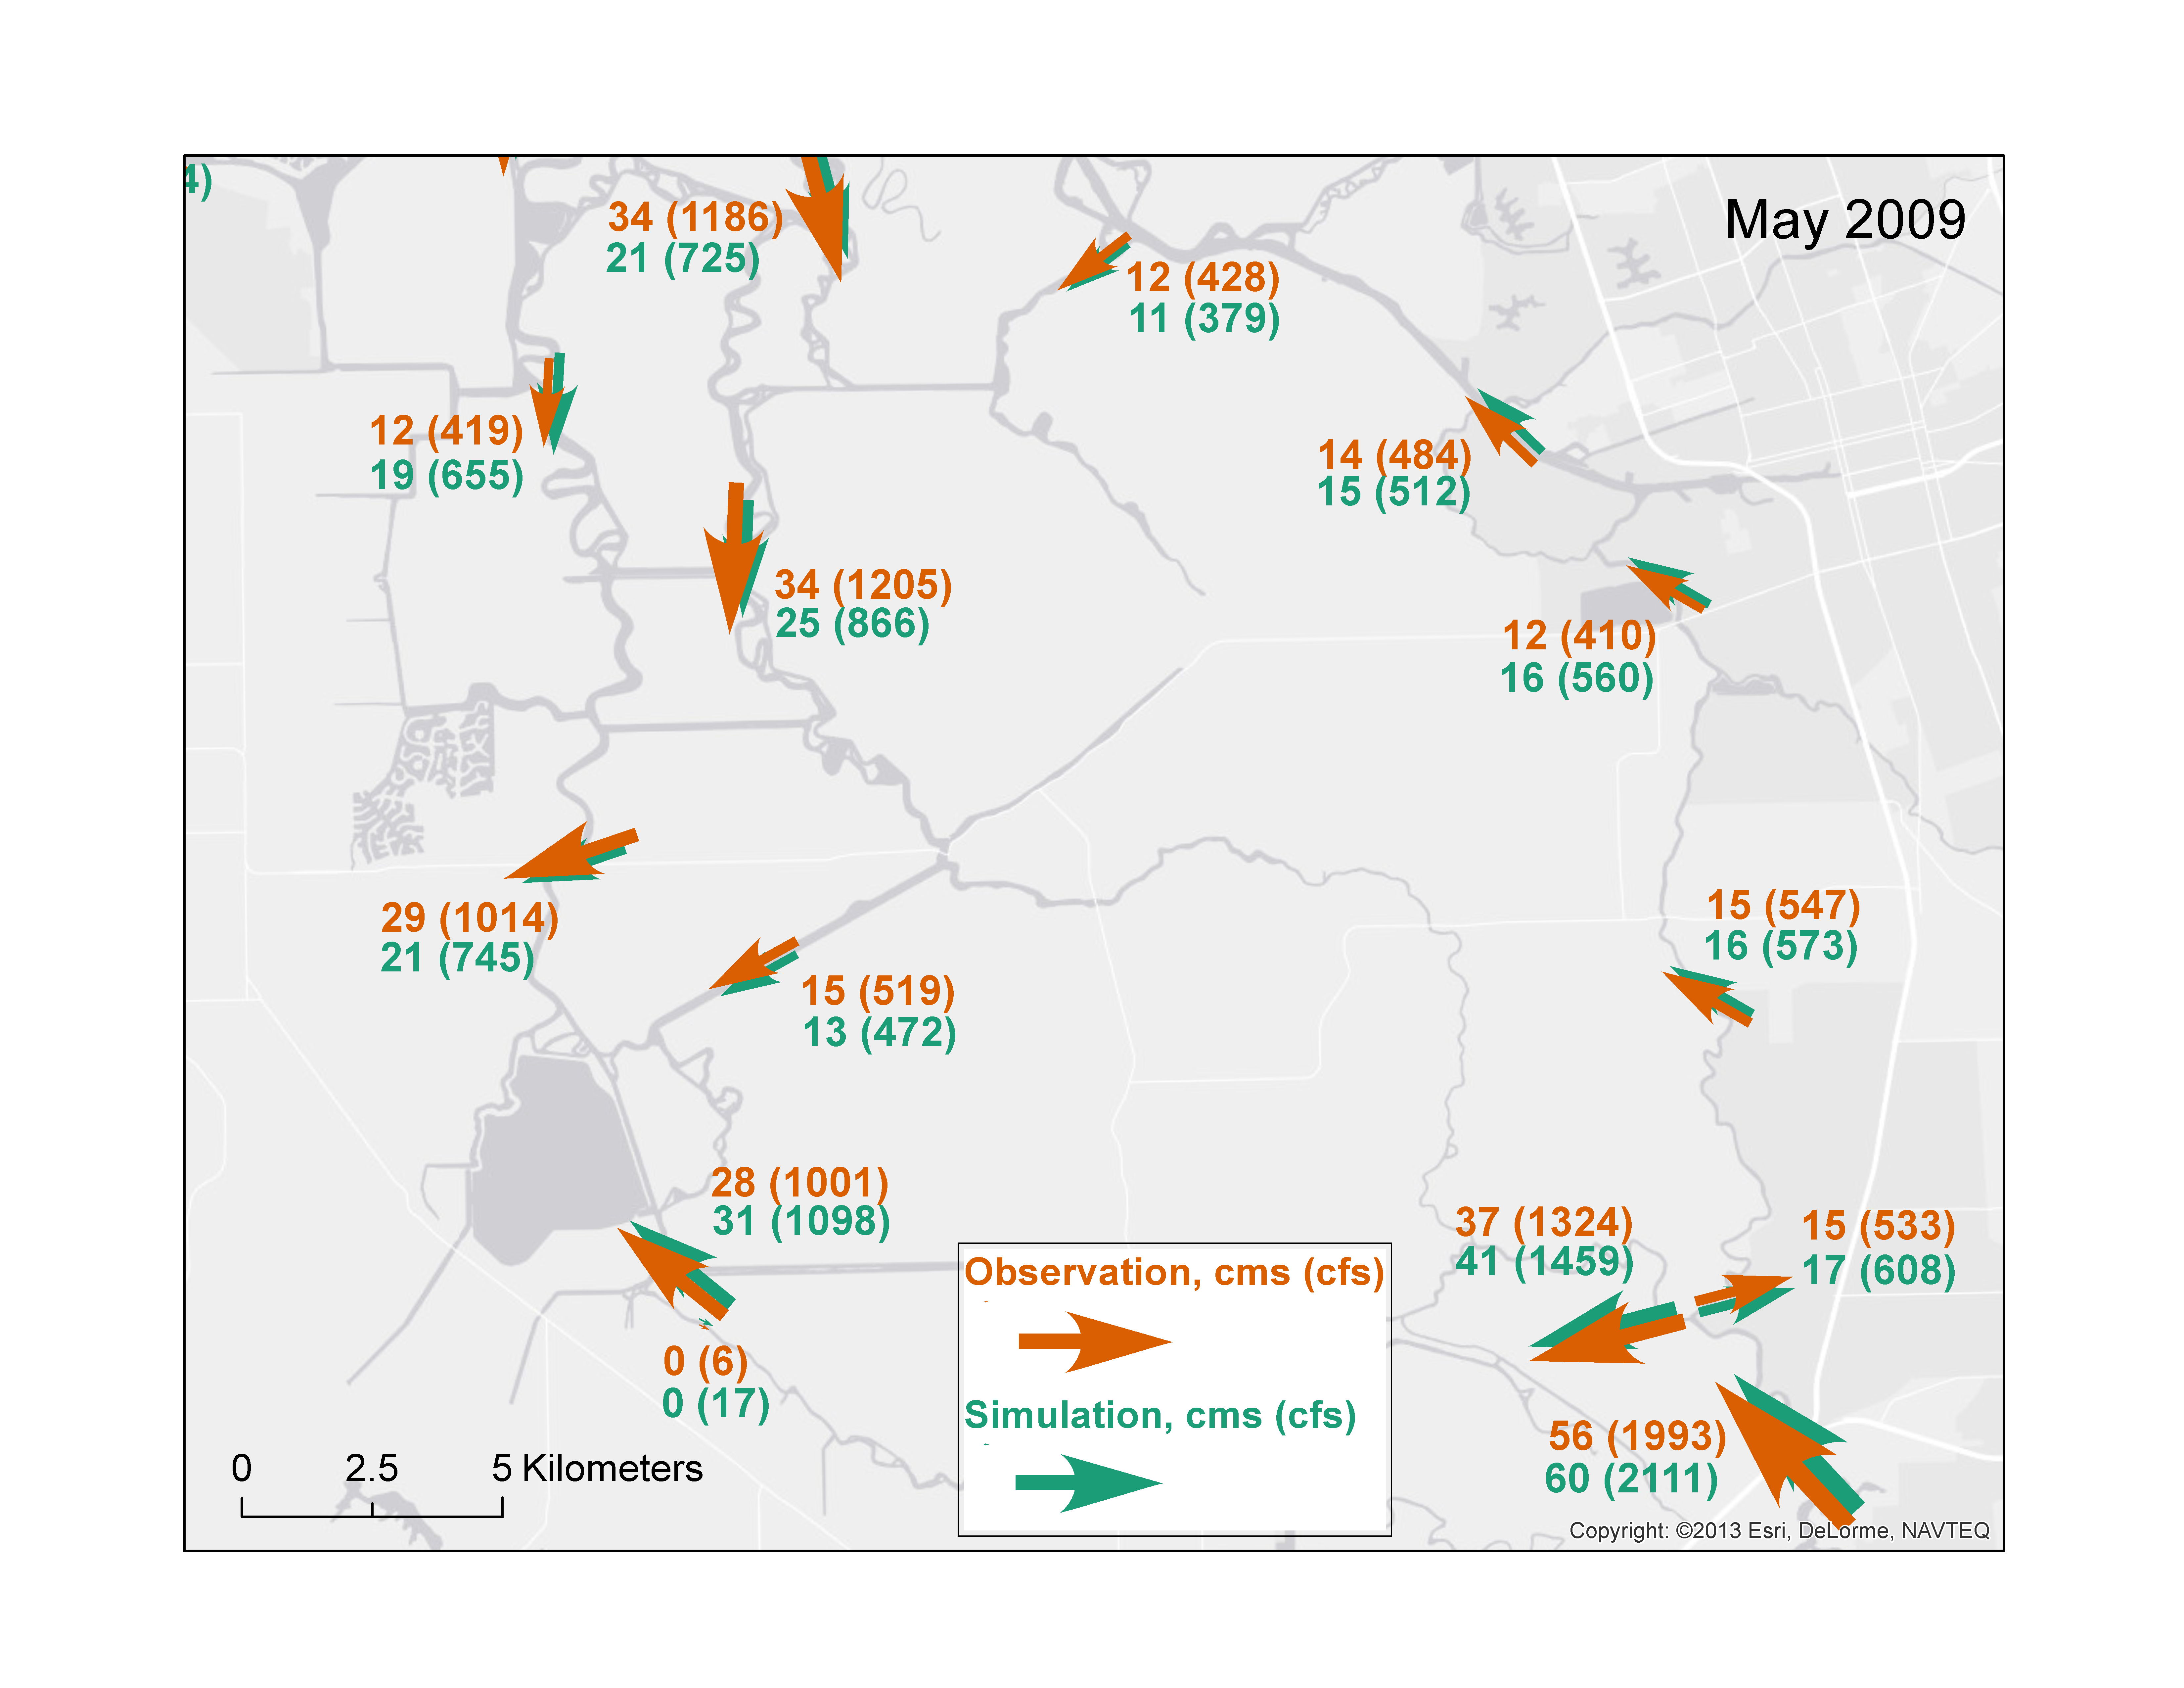
\includegraphics[width=\textwidth]{image/residual_flow_south_delta_64a_may}
	\caption{South Delta monthly residual flow, May 2009. Units are cms (cfs in parentheses).}
	\label{fig:resid_south_may}
\end{figure}
	
\section{Salinity Results}
  \subsection{Monitoring stations}
  \subsection{Surface-bottom stratification}
	\subsection{USGS Cruise CTD casts}

\section{Model sensitivity}
  \subsection{Mesh alteration}
	\subsection{Mesh refinement}
	\subsection{Friction change}
	\subsection{Mass conservation}
  \subsection{Vertical closure}
	\subsection{Atmospheric input}
	\subsection{Boundary Reflection}
  \subsection{Upper water surface and vel flareups}